\chapter{Projekt systemu}
\label{cha:projektSystemu}
Rozdział ten w 3 podrozdziałach przedstawia koncepcję implementowanej aplikacji. W podrozdziale pierwszym opisany jest system, w drugim znajduje się specyfikacja wymagań, a w trzecim model systemu. Dokumentacja projektu została częściowo oprata na szablonie dokumentacji projektu stworzonym przez dr Piotra Szweda \cite{DOC01}.
\section{Opis systemu}
W tym podrozdziale opisany jest cel systemu, jego granice, lista możliwości systemu oraz jego użytkownicy. Ponadto za pomocą diagramów aktywności przedstawione jest działanie aplikacji.
\subsection{Cel projektu}
Celem projektu jest implementacja serwisu internetowego dedykowanego dla studentów w architekturze SOA. Głównym zadaniem serwisu ma być możliwość przechowywania plików oraz udostępnianie ich innym użytkownikom. Ponadto każdy z użytkowników będzie mógł korzystać z dedykowanego dla niego kalendarza, w którym może zapisywać ważne wydarzenia. Oprócz opisanych wcześniej funkcji użytkownik za pomocą strony powiadomień będzie mógł się dowiedzieć o nadchodzących wydarzeniach oraz o udostępnionych dla niego plikach.

\subsection{Użytkownicy}
Grupę użytkowników stanowią wszyscy korzystającyz serwisu, z wyszczególnieniem:
\begin{itemize}
	\item \textbf{Użytkownik} - Docelowym użytkownikiem serwisu jest student potrzebujący dodać lub uzyskać dostęp do pliku poprzez udostępnienie od innych użytkowników serwisu. Nie jest warunkiem koniecznym, aby użytkownik był studentem.
	\item \textbf{Administrator} - Użytkownik posiadający szystkie uprawnienia, takie jak usówanie użytkowników oraz wgląd do wszystkich plików w systemie.
\end{itemize}

\subsection{Granice systemu}
Granicą systemu dla użytkownika jak i dla administratora będzie strona internetowa aplikacji. Zawarty będzie tam dostęp do wszystkich funkconalności systemu. Administrator dodatkowo będzie miał dostęp do specjalnego panelu za pomocą którego będzie mógł zarządzać kontami wszystkich użytkowników.

Wejścia w systemie:
\begin{itemize}
	\item formularz nowego konta – użytkownik wypełnia dane: login, hasło, imie, nazwisko, adres e-mail,
	\item formularz logowania – zalogowanie się do systemu za pomocą loginu i hasła użytkownika,
	\item formularz edycji konta – zmiana danych użytkownika,
	\item formularz nowego pliku – załączonik oraz opcjonalnie tytuł i opis pliku,
	\item formularz edycji pliku - zmiana załącznika, tytułu lub opisu,
	\item formularz udostępnienia pliku - login użytkownika, któremu ma być udostępniony wybrany plik,
	\item formularz nowego wydarzenia - wybrana data, nazwa wydarzenia oraz opcjonalny opis,
	\item formularz edycji wydarzenia - nowe dane do wybranego wydarzenia,
\end{itemize}
Wyjścia w systemie:
\begin{itemize}
	\item Strona powiadomień - na tej stronie znajdować się będą informacje o udostępnionych plikach oraz o przypomnienia o nadchodzących wydarzeniach.
	\item Strona przeglądania własnych plików - użytkownik na tej stronie może przeglądać dodane przez siebie pliki,
	\item Strona przeglądania udostępnionych plików - tutaj użytkownik będzie mógł przeglądać pliki mu udostępnione,
	\item Strona kalendarza - Strona odpowiedzialna za wyświetlanie kalendarza.
\end{itemize}
\subsection{Lista możliwości}
\label{listaFun}
Lista wymagań funkcjonalnych:
\begin{itemize}
	\item Logowanie,
	\item Wylogowanie,
	\item Rejestracja,
	\item Zarządzanie kontem,
	\item Zarządzanie materiałami,
	\item Pobieranie pliku,
	\item Udostępnianie pliku,
	\item Zarządzanie kalendarzem,
	\item Otrzymywanie powiadomień,
\end{itemize}

Dodatkowe funkcje administratora:
\begin{itemize}
	\item Zarządzanie kontami użytkowników.
\end{itemize}

Na kolejnych stronach zostały przedstawione diagramy czynności typowych akcji.

	
\section{Specyfikacja i analiza wymagań}
Dzięki analizie wymagań funkcjonalnych możemy zidentyfikować oczekiwane zachowania budowanego systemu. Wymaganie funkcjonalne jest to „stwierdzenie, jakie usługi ma oferować system, jak ma reagować na określone dane wejściowe oraz jak ma się zachowywać w określonych sytuacjach. W niektórych wypadkach wymagania funkcjonalne określają, czego system nie powinien robić” \cite{DOC02}. W tym podrozdziale opisane zostaną lista wymagań wunkonalnych oraz niefunkcjonalnych oraz przedstawiony zostanie diagram przypadków użycia z dołączonymi scenariuszami.
\subsection{Wymagania oprogramowania}
Wymagania funkcjonalne zostały wypisane w podpunkcie \ref{listaFun}.
Wymagania niefunkcjonalne:
\begin{enumerate}
	\item Wymaganie organizacyjne:
		\begin{itemize}
			\item Implementacji : językiem programowania jest Java,
			\item Użyteczności : Interfejs graficzny użytkownika jest przejrzysty i łatwy do przyswojenia,
		\end{itemize}
	\item Wymagania zewnętrzne:		
		\begin{itemize}
			\item Poufności - Projekt przestrzega wymagań prawnych ustanowionych w Ustawie o Ochronie Danych Osobowych.
			\item Bezpieczeństwa : System nie pozwala użytkownikom na nieautoryzowany dostęp do bazy danych
		\end{itemize}
\end{enumerate}
\subsection{Ryzyka operacyjne}
Ryzykiem w implementowanym systemie może być niedostateczne zabezpieczenie bazy danych lub pojawienie się nieobsłużonych błędów.
//TODO: Poszukać i dodać tu jeszcze cos
\subsection{Przypadki użycia}
Dzięki przypadkom użycia możemy okeślić jak użytkownik będzie korzystał z systemu. Dzięki diagramowi możemy zobaczyć jakie czynności może wykonywać dany użytkownik \cite{DOC03}. Opisy czynności zawartych na diagramie znajdują się w scenariuszach przypadków użycia.

Poniższe diagramy prezentują możliwe interakcje użytkowników z systemem.
\begin{figure}[h]
	\centering
	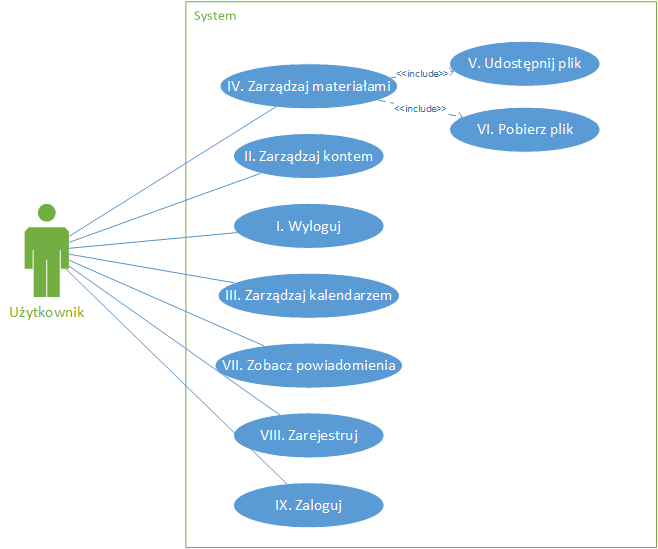
\includegraphics[scale=0.7]{UseCaseUser}
	\caption{\label{fig:caption_01}Diagram przypadków użycia dla użytkownika}
\end{figure}
W poniższym diagramie pominięto przypadki użycia, które posiada zwykły użytkownik, lecz nie należy zapominać, że administrator również je posiada.
\begin{figure}[h]
	\centering
	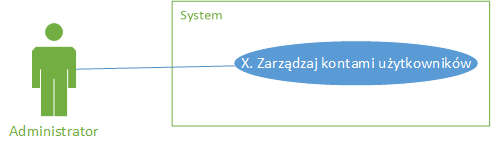
\includegraphics[scale=0.7]{UseCaseAdmin}
	\caption{\label{fig:caption_01}Diagram przypadków użycia dla administratora}
\end{figure}

Scenariusze przypadków użycia:
\begin{table}[h]
\centering
\caption{Wyloguj}
\label{wyloguj}
\begin{tabular}{|p{7cm}|p{7cm}|}
  \hline 
  \textbf{Aktorzy:} & Użytkownik, Administrator\\
  \hline
  \textbf{Zakres:} & System \\
	\hline
  \textbf{Poziom:} & Sytemowowy \\
	\hline
  \textbf{Udziałowcy i ich cele: } & Użytkownik chce się wylogować. \\
	\hline
  \textbf{Zdarzenie wyzwalające } & Użytkownik wciska przycisk “Wyloguj”. \\
	\hline
  \textbf{Warunki wstępne: } & Użytkownik jest zalogowany.
 \\
	\hline
  \textbf{Warunki końcowe dla sukcesu:} & Użytkownik jest wylogowany.
 \\
	\hline
  \textbf{Warunki końcowe dla niepowodzenia:} & Użytkownik jest zalogowany. \\
  \hline
\end{tabular} 
\end{table}
\newpage
\textbf{Scenariusz główny:} \\
1. Użytkownik wciska przycisk wyloguj widoczny w prawym górnym rogu strony. \\
2. Pojawia się okno z napisem: “Czy na pewno chcesz się wylogować?” \\
3. Użytkownik wciska przycisk “tak”. \\
4. Użytkownik jest wylogowany i przekierowany na stronę główną systemu. \\
\textbf{Scenariusz alternatywany: \\
} 
3.a. Użytkownik wciska “nie”. \\
3.a.1. Okno z napisem znika, użytkownik dalej jest zalogowany. \\

\begin{table}[h]
\centering
\caption{Zarządzaj kontem}
\label{zarzadzajkontem}
\begin{tabular}{|p{7cm}|p{7cm}|}
  \hline 
  \textbf{Aktorzy:} & Użytkownik, Administrator\\
  \hline
  \textbf{Zakres:} & System \\
	\hline
  \textbf{Poziom:} & Sytemowowy \\
	\hline
  \textbf{Udziałowcy i ich cele: } & Użytkownik chce zmienić login lub hasło. \\
	\hline
  \textbf{Zdarzenie wyzwalające } & Użytkownik wciska przycisk “Zarządzaj kontem”. \\
	\hline
  \textbf{Warunki wstępne: } & Użytkownik jest zalogowany.\\
	\hline
  \textbf{Warunki końcowe dla sukcesu:} & Login lub hasło użytkownika są zmienione.\\
	\hline
  \textbf{Warunki końcowe dla niepowodzenia:} & Login lub hasło użytkownika nie są zmienione. \\
  \hline
\end{tabular} 
\end{table}

\section{Model systemu}
nad tym tytulem pomyslec!\newline
\subsection{Architektutra systemu}
- najpierw napisac ze soa\newline
- zastanowic sie czy tutaj opis soa czy we wstepie, ale chyba we wstepie, tutaj jedynie można wspomiec ze wczesniej opisany w punkcie X.x.\newline
- Diagram \newline
- byc moze opis

\subsection{Model bazy danych}
- tutaj jakis ladny wstep.\newline
- MODEL ERD - ostateczny \newline

\subsection{Model klas}
- rowniez jakis ladny wstep \newline
- No i diagram klas tutaj ładnie sklepać trzeba będzie \newline

\subsection{Diagramy sekwencji}
- Wstep, ze to wynika z diagramu klas, cos ładnego o diagramach sekwencji - tutaj moze sie wykładami szweda posłużyć \newline
- No i wklepac diagramy sekwencji - moze nie bedzie tak zle jak już beda diagramy klas \newline
\section {Projekt interfejsu?}
Nad tym sie zastanowic czy to robic czy dac dupie siana

